\section{Colisões}\label{section:pncg_colisoes}

O intervalo maximal de soluções do PNCG não necessariamente se estende para toda a reta, pois existem circunstâncias em que a solução é interrompida abruptamente. Um exemplo de caso é quando duas trajetórias se interceptam em um dado instante comum, o que fisicamente significa que dois corpos colidiram. 

Lidar com essas situações é também necessário do ponto de vista numérico, pois muitas vezes não se pretende encerrar uma simulação quando dois corpos colidirem. Além disso, mesmo aproximações muito intensas são capazes de instabilizar numericamente os métodos devido aos erros de ponto flutuante, então, ainda que duas trajetórias não colidam exatamente, pode ser numericamente interessante lidar com a aproximação supondo que houve colisão.

De fato, tais situações de aproximação são de maior interesse, pois é conhecido que o conjunto de condições iniciais que leva a uma colisão em tempo finito tem medida de Lebesgue zero \citep{Saari1971}. Então, embora isso não implique na impossibilidade de que ocorram, colisões \textit{verdadeiras} são raras.

Existem algumas formas de tratar esses casos, como por meio de regularizações ou mesmo com amortecedores no potencial, como será discutido na seção \ref{section:simulacao_colisoes}. Uma possibilidade aqui proposta é a de adicionar colisões perfeitamente elásticas. As colisões perfeitamente elásticas (ou CPE) são aquelas em que não há deformação dos objetos e a energia cinética é conservada. Essa é uma possível vantagem sobre os outros métodos, uma vez que não compromete a estrutura simplética de sistemas hamiltonianos.

Uma abordagem consiste em definir um parâmetro de densidade $\rho$, e uma vez que cada corpo tem massa, a densidade definirá um volume. Na suposição de que os corpos são perfeitamente esféricos, tem-se o raio
\begin{equation}
    r = \sqrt[3]{\dfrac{3 m}{4 \pi \rho}}.
\end{equation}

Além disso, um critério para garantir que dois corpos próximos de massas $m_1$ e $m_2$, posições $\vet q_1$ e $\vet q_2$ e velocidades $\vet v_1$ e $\vet v_2$, estão em rota de colisão é verificar se
\begin{equation*}
    \prodint{\vet q_2 - \vet q_1}{\vet v_2 - \vet v_1} \leq 0.
\end{equation*}

% Comecar a falar da fisica das colisoes

A dinâmica pós-colisão é definida da maneira que segue. Sejam as massas, posições e velocidades como anteriormente. Sejam também $\vec \pi$ o plano tangente de contato e $\vet N$ o versor normal ao plano:
\begin{equation}
    \vet N = \dfrac{\vet q_2 - \vet q_1}{\norma{\vet q_2 - \vet q_1}} = (n_1, n_2, n_3).
\end{equation}

\begin{figure}[H]
    \centering
    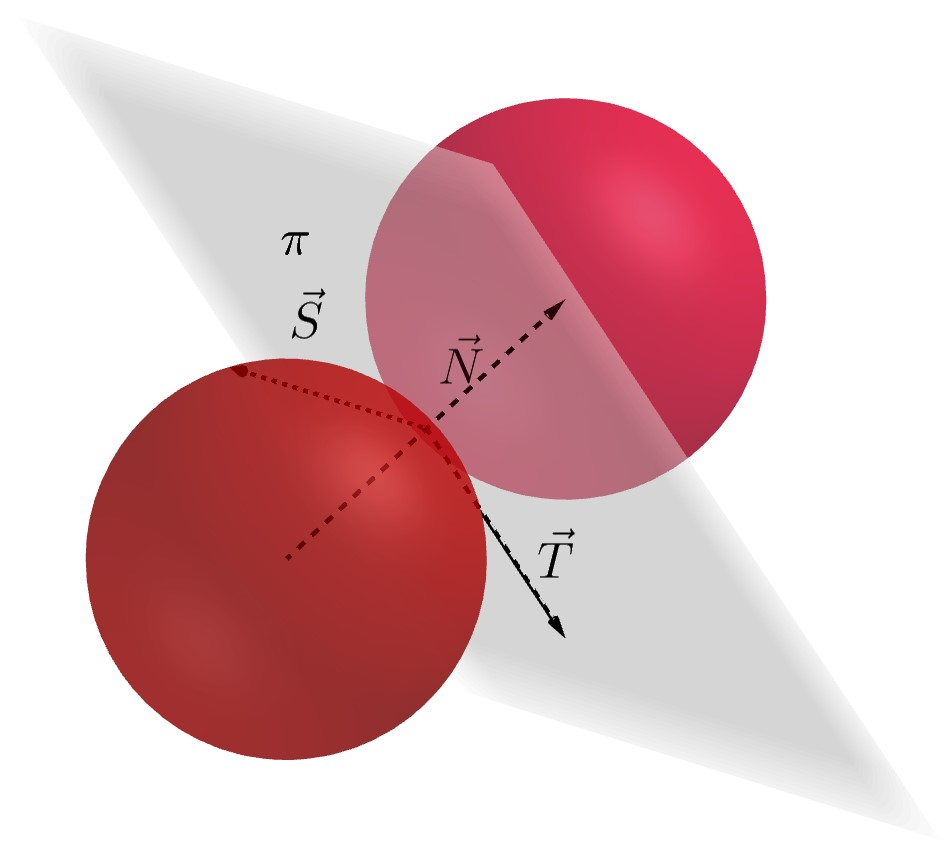
\includegraphics[width=4cm]{tcc/img/colisao_corrigida.jpg}
    \caption{Colisão entre dois corpos, plano tangente $\vet \pi$ e versores.}
    \label{fig:colisao-3d}
\end{figure}

Para obter os versores geradores do plano, basta tomar, por exemplo, os vetores
\begin{equation*}
    \vet T = \dfrac{(n_3, n_3,-n_1 - n_2)}{\norma{(n_3, n_3,-n_1 - n_2)}},
    \quad
    \vet S = \dfrac{\vet N \times \vet T}{\norma{\vet N \times \vet T}},
\end{equation*}
como na figura \ref{fig:colisao-3d}. Observe que $\vet T$ não é bem definido, uma vez que $n_1 = -n_2$ e $n_3 = 0$ gera $\vet T = \vet 0$. Na ocorrência desse caso, uma solução possível é utilizar outro vetor $\vet T$:
\begin{equation*}
    \vet T = \dfrac{(-n_2, n_1, 0)}{\norma{(-n_2, n_1, 0)}}.
\end{equation*}
Supondo que não ocorrem colisões reais, isto é, que $\vet N \neq \vet 0$ (o que, numericamente, é uma suposição válida), definimos $\vet S$ da mesma forma e o método que segue se mantém.

Com isso, as velocidades podem ser decompostas em relação ao plano tangente e em relação ao vetor normal:
\begin{align*}
    \vet v_1 &= \vet v_1^{\vet \pi} + v_1 \vet N,
    \\
    \vet v_2 &= \vet v_2^{\vet \pi} + v_2 \vet N.
\end{align*}

Uma vez que o sistema não contém rotações individuais, em uma colisão não há forças atuando nas direções do plano tangente, então a única alteração se dá nas componentes normais. Sendo $v_1'$ e $v_2'$ as novas velocidades normais, a colisão ser perfeitamente elástica implica na conservação do momento linear total e da energia cinética:
\begin{equation}\label{eq:colisoes_conservacao}
    \begin{cases}
        m_1 v_1 + m_2 v_2 = m_1 v_1' + m_2 v_2', \\
        m_1 v_1^2 + m_2 v_2^2 = m_1 v_1'^2 + m_2 v_2'^2.
    \end{cases}
\end{equation}

Do sistema de equações (\ref{eq:colisoes_conservacao}), decorre que
\begin{align*}
    v_1' &= \dfrac{v_1 (m_1 - m_2) + 2 m_2 v_2}{m_1 + m_2}, \\
    v_2' &= \dfrac{v_2 (m_2 - m_1) + 2 m_1 v_1}{m_1 + m_2}.
\end{align*}

Dessa forma, as novas velocidades após a colisão são:
\begin{align*}
    \vet v_1' = \vet v_1^{\vet \pi} + v_1' \vet N, \\
    \vet v_1' = \vet v_1^{\vet \pi} + v_1' \vet N.
\end{align*}

\begin{figure}[H]
    \centering
    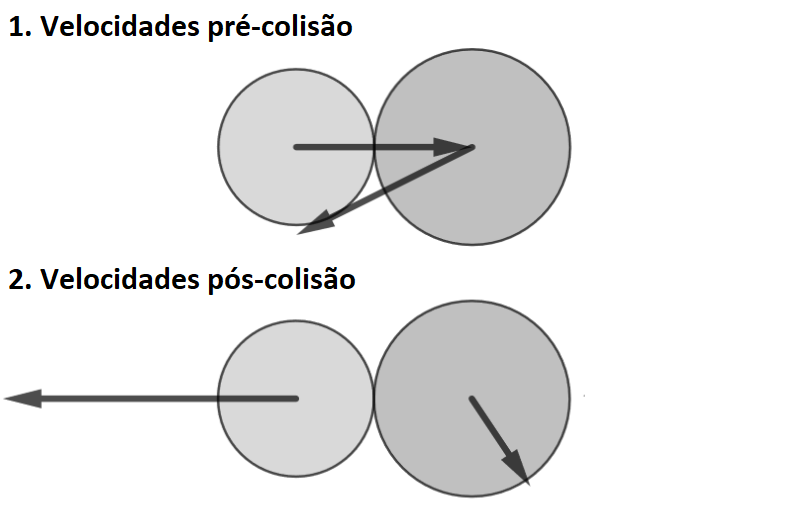
\includegraphics[width=8cm]{img/colisao_exemplo.png}
    \caption{Exemplo de colisão. Os tamanhos diferentes indicam massas diferentes.}
    \label{fig:colisao_exemplo}
\end{figure}

Na figura \ref{fig:colisao_exemplo} tem-se um exemplo de colisão entre dois corpos com massas diferentes. Como esperado, um corpo de massa menor sai da colisão com mais velocidade (e com sentido oposto), enquanto um de massa maior sai com menos velocidade (e com componente normal também no sentido oposto).